%% Standalone source of one report figure. Rebuild: pdflatex -output-directory=.. fig-04-pothole-states.tex
\documentclass[11pt]{standalone}
\usepackage[T1]{fontenc}
\usepackage[utf8]{inputenc}
\usepackage{lmodern}
\usepackage{microtype}
\usepackage{amsmath,amssymb}
\usepackage{xcolor}
\usepackage{tikz}
\usetikzlibrary{arrows.meta,positioning,shapes.geometric,fit,calc,backgrounds}
\usepackage{pgfplots}
\usepackage{pgfplotstable}
\pgfplotsset{compat=1.18}
\setlength{\textwidth}{472.31595pt}  %% = the report's text width, so widths given in \textwidth match
\definecolor{gmblue}{HTML}{0B3D6E}
\definecolor{gmok}{HTML}{1E7B34}
\definecolor{gmwarn}{HTML}{B35C00}
\definecolor{gmbad}{HTML}{A32020}
\definecolor{gmgrey}{HTML}{5A5F66}
\definecolor{gmlight}{HTML}{EEF3F8}
\definecolor{gmteal}{HTML}{1B7A8C}
\newcommand{\done}{\textcolor{gmok}{\textbf{Done}}}
\newcommand{\partly}{\textcolor{gmwarn}{\textbf{Partly}}}
\newcommand{\pending}{\textcolor{gmbad}{\textbf{Pending}}}
\newcommand{\pass}{\textcolor{gmok}{\textbf{PASS}}}
\newcommand{\fail}{\textcolor{gmbad}{\textbf{FAIL}}}
\newcommand{\code}[1]{\texttt{\small #1}}
\newcommand{\INR}{INR~}
\newcommand{\gbar}[5]{\fill[#5] (#1,-#3+0.32) rectangle (#2,-#3-0.32);
  \node[anchor=east,font=\scriptsize] at (-0.3,-#3) {#4};}

\tikzset{
  box/.style={draw=gmblue, rounded corners=3pt, fill=gmlight, align=center, font=\small, inner sep=5pt,
              minimum height=9mm},
  gstep/.style={draw=gmblue, rounded corners=3pt, fill=white, align=center, font=\footnotesize, inner sep=4pt,
               text width=27mm, minimum height=11mm},
  st/.style={draw=gmblue, rounded corners=6pt, fill=gmlight, font=\scriptsize\ttfamily, inner sep=3pt,
             minimum height=6mm},
  arr/.style={-{Stealth[length=2.2mm]}, thick, gmblue},
  darr/.style={-{Stealth[length=2mm]}, gmgrey, dashed},
}

\begin{document}
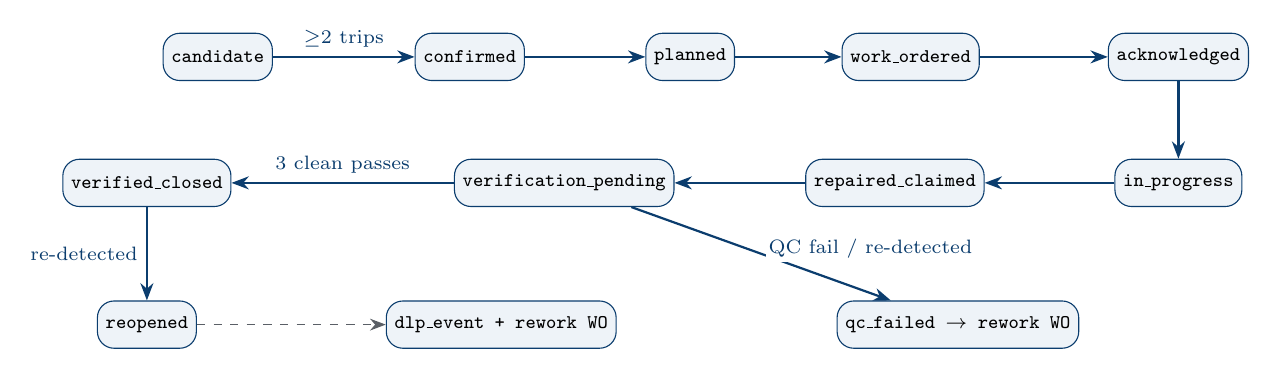
\begin{tikzpicture}[lbl/.style={font=\scriptsize, fill=white, inner sep=1pt}]
  \node[st] (c)  at (0,0)     {candidate};
  \node[st] (cf) at (3.2,0)   {confirmed};
  \node[st] (pl) at (6.0,0)   {planned};
  \node[st] (wo) at (8.8,0)   {work\_ordered};
  \node[st] (ak) at (12.2,0)  {acknowledged};
  \node[st] (ip) at (12.2,-1.6) {in\_progress};
  \node[st] (rc) at (8.6,-1.6)  {repaired\_claimed};
  \node[st] (vp) at (4.4,-1.6)  {verification\_pending};
  \node[st] (vc) at (-0.9,-1.6) {verified\_closed};
  \node[st] (ro) at (-0.9,-3.4) {reopened};
  \node[st] (dlp) at (3.6,-3.4) {dlp\_event + rework WO};
  \node[st] (qf) at (9.4,-3.4)  {qc\_failed $\rightarrow$ rework WO};
  \draw[arr] (c)--node[lbl, above=2pt]{$\geq$2 trips}(cf);
  \draw[arr] (cf)--(pl); \draw[arr] (pl)--(wo); \draw[arr] (wo)--(ak);
  \draw[arr] (ak)--(ip); \draw[arr] (ip)--(rc); \draw[arr] (rc)--(vp);
  \draw[arr] (vp)--node[lbl, above=2pt]{3 clean passes}(vc);
  \draw[arr] (vc)--node[lbl, left=2pt]{re-detected}(ro);
  \draw[darr] (ro)--(dlp);
  \draw[arr] (vp) -- node[lbl, right=6pt, pos=0.45]{QC fail / re-detected} (qf);
\end{tikzpicture}
\end{document}
